% ICMC 2006 paper template for Latex2e.

% Points to note:
%    Please use \paragraph instead of \subsubsection -- see discussion below.
%    See comments in the References section on how to do citations.

\documentclass[10pt,letterpaper]{article}
\usepackage{graphicx}
\usepackage{subfigure}
\usepackage{fullpage}
\usepackage{times}
\usepackage{chicago}                    % for "(Author, year)" cite style.
\usepackage{indentfirst}                % indent para after headings.
% \usepackage{url}                      % (handy if you reference a URL.)

\setlength{\oddsidemargin}{-0.25in}     % Latex has one-inch "driver margin"
% \setlength{\evensidemargin}{-0.25in}  % (shouldn't be necessary)
\setlength{\textwidth}{7in}             % 8.5 - 2*0.75 

%\clubpenalty=9999
%\widowpenalty=9999

\setlength{\columnsep}{0.25in}
\setlength{\parindent}{0.2in}
\setlength{\abovecaptionskip}{2pt}
\setlength{\belowcaptionskip}{-8pt}

\newenvironment{myitemize}{\begin{list}{$\bullet$}
{\setlength{\itemsep}{.25pt}\setlength{\parsep}{0pt}\settowidth{\leftmargin}{$\bullet$~}}}
{\end{list}}

\raggedbottom                           % better than inter-para spaces, I say.


\begin{document}

\twocolumn

\title{\textbf{Musical Tapestry: Re-composing Natural Sounds}}
\author{
Ananya Misra, Perry R. Cook$^{\dag}$, Ge Wang\\
Department of Computer Science ($^{\dag}$also Music), Princeton University \\
\{amisra, prc, gewang\}@cs.princeton.edu\\
}
\date{}     % no date
\maketitle

\pagestyle{empty}          % no page numbers.
\thispagestyle{empty}      % yes, that includes not on the first page, either.

% do abstract by hand -- \begin{abstract} wouldn't conform to the guidelines.

\begin{center}
\large{\textbf{Abstract}}
\end{center}
% there's this annoying little indent here I can't properly eliminate, so...
\hspace*{-0.1in}                       % hackily cancel it out.
\noindent
\textit{
A system to aid composition with analysis, transformation,
and resynthesis of natural sounds is described.  Sinusoidal 
analysis is used to isolate and extract deterministic sounds, 
and transients are also isolated/extracted, leaving the 
stochastic background sound which is parameterized 
by wavelet tree analysis.   All of these components 
become templates for the synthesis phase, which is 
controlled 1) by placing templates on timelines or in groups,
2) by real-time manipulation of parameters,
and 3) via scripting using the ChucK language.  
The result is a flexible ``workbench'' for doing modern day
musique concr\`{e}te or acousmatic composition, sound 
design, and other sonic sculpting tasks.
}

\begin{figure*}[tbh!]
\centering
    \includegraphics[width=.95\textwidth]{teaser.pdf}
    \caption{\textbf{Creating musical tapestries}.  User-selected regions of input sounds (left) are 
    analyzed into reusable templates, which are separately transformed and resynthesized into
    new sounds (right). Numbered diamonds (right) correspond to instances of original sound
    components (circled, left).  The framework allows flexible control at every stage in the process.} 
    \label{fig:teaser}
\end{figure*}

\section{Motivation}

\noindent
Around 1950, Pierre  Schaeffer  developed  musique
concr\`{e}te ~\cite{Schaeffer50,Schaeffer52}.  Unlike traditional music,
musique concr\`ete starts with existing or concrete rec\-orded sounds,
which are organized into abstract musical structures. The existing
recordings often include natural and industrial sounds that are not
conventionally musical, but can be manipulated to make music, either by
editing magnetic tape or now more commonly through digital sampling.
Typical manipulations include cutting, copying, reversing, looping and
changing the speed of recorded segments.

Today, several other forms of electronic/electroacoustic music also
involve manipulating a set of recorded sounds. Acousmatic
music~\cite{Dhomont95}, for instance, evolved from musique concr\`ete
and refers to compositions designed for environments that emphasize the
sound itself rather than the performance-oriented aspects of the piece.

The acoustic ecology~\cite{Schafer77} movement gave rise to soundscape
composition~\cite{Truax02} or the creation of realistic
soundscapes from recorded environmental audio. One of the key features
of soundscape composition, according to Truax, is that ``most pieces can
be placed on a continuum between what might be called `found sound' and
`abstracted' approaches.'' However, while ``contemporary signal
processing techniques can easily render such sounds unrecognizable and
completely abstract,'' a soundscape composition piece is expected to
remain recognizable even at the abstract end of the continuum.

Sound designers for movies, theater and art often have a related goal of
starting with real world sounds and creating emotionally evocative sound
scenes, which are still real, yet transformed and transformative.
Classic examples include mixing a transformed lion's roar with other
sounds to accompany the wave sounds in \textit{The Perfect Storm}, and
incorporating a helicopter theme into the sound design for \textit{Black
Hawk Down}~\cite{Rudy04}.  These sound designers are ``sound sculptors''
as well, but transform sounds to enhance or create a sense of reality,
rather than for purely musical purposes.

Artists from all of the above backgrounds share the process
of manipulating recordings, but aim to achieve different
effects. We present a single framework for starting with
recordings and producing sounds that can lie anywhere on a
`found' to `unrecognizable' continuum. `Found' sounds can
be modified in subtle ways or extended indefinitely, while
moving towards the `unrecognizable' end of the spectrum unleashes
a range of manipulations beyond time-domain techniques.
In fact, the same set of techniques applies throughout
the continuum, differing only in how they are used. We call
this framework TAPESTREA: Techniques and Paradigms for
Expressive Synthesis, Transformation and Rendering of Environmental
Audio.

The TAPESTREA system integrates sinusoidal analysis, stochastic background
modeling, transient detection, and a new class of user interface that
lends itself to any composition that originates in recorded
environmental audio. This envelopes a novel form of musique concr\`ete
that extends to manipulations in the frequency as well as time domain.
Advantages of the TAPESTREA approach include:
\begin{myitemize}
\setlength{\itemsep}{2pt}
\item TAPESTREA lets the sound sculptor select a region in both 
time and frequency, essentially specifying, ``Give me \textit{this} part of
\textit{that} sound,'' to extract a reusable 
\textit{sound template}. 
Existing techniques for manipulating
recordings -- both time-domain-centric methods and spectrally oriented 
approaches, such as the phase vocoder -- support only moderate transformations.
% are often time-domain-centric, with even spectrally oriented
%tools like the phase vocoder supporting only moderate transformations,
TAPESTREA leverages sinusoidal modeling to enable high-quality,
potentially extreme, time and frequency transformations on appropriate 
template types.
\item TAPESTREA defines three fundamental types of sound components / templates, based
on the modeling techniques for which they are best suited. {\it Deterministic}
(sinusoidal), {\it transient}, and {\it stochastic background} components are
modeled separately, using methods to which they are most amenable,
leading to specialized control and more powerful transformations on 
each type.
\item To realize these ideas, TAPESTREA provides a set of interfaces 
that allow the sound designer or composer to assert parametric  
control over each phase in the process, from component extraction to the 
final resynthesis. 
%Templates can be manipulated individually and in groups,
%modeling both single sound and group characteristics. - moved to synthesis
\end{myitemize}

TAPESTREA manipulates sounds in several phases (Figure \ref{fig:teaser}). In the analysis
phase, the sound is separated into reusable components that correspond to
individual foreground events or background textures. In the synthesis phase,
these components are transformed, combined and re-synthesized using
time- and freq\-uency-domain techniques that can be controlled on multiple
levels. While we highlight the synthesis methods here, the analysis
phase is also integral as it enables the most flexible means for dealing
with real-world sonic material.

\section{Related Work}

Related techniques used for musical composition include spectral modeling
synthesis~\cite{Serra89} and granular 
synthesis~\cite{Truax90,Roads02}. Spectral modeling synthesis 
separates a sound into sinusoids and
noise, and was originally used for modeling instrument sounds. Granular
synthesis, in contrast, functions in the time-domain and involves
continuously controlling very brief sonic events or sound grains. TAPESTREA
employs aspects of both, using separation techniques on environmental sounds
and controlling the temporal placement of resulting events.

Another technique used in TAPESTREA is an extension of a wavelet tree
learning algorithm~\shortcite{Dubnov02} for sound texture synthesis. This
method performs a wavelet decomposition on a sound clip and uses machine
learning on the wavelet coefficients to generate similar non-repeating sound
texture. The algorithm works well for sounds that are mostly stochastic, but
can break extended pitched portions in objectionable ways. It can also be 
slow in its original form. TAPESTREA takes advantage of this technique by 
improving the speed of the algorithm, and only using it on the types of 
(non-deterministic) sound for which it works well.

\section{Analysis Phase}

TAPESTREA starts by separating a recording into \textit{deterministic
events} or stable sinusoidal components of the
sound, \textit{transient events} or brief noisy bursts of energy, and the
remaining \textit{stochastic background} or din. This separation can
be parametrically controlled and takes place in the analysis
phase.  In a sense, boundaries between component types are not rigid,
but are interactively defined by the user.

The analysis interface is shown in the accompanying figures. A loaded
sound is simultaneously displayed as a waveform
and a spectrogram (Figure \ref{fig:ui_specgram}). The spectrogram
display can also be toggled with a frame-by-frame spectrum view (Figure
\ref{fig:ui_spectrum}). Selecting a rectangle on the spectrogram, or
selecting an analysis region on the waveform and the frame-by-frame
spectrum, limits the analysis to the associated time and frequency
ranges, facilitating the selection and extraction of specific events. 

\begin{figure}[h]
  \begin{center}
%    \framebox[7cm]{\rule[-5mm]{0cm}{5cm} }
    \includegraphics[width=1\columnwidth]{ui_specgram_w.pdf}
    \caption{Spectrogram view in analysis face.} 
    \label{fig:ui_specgram}
  \end{center}
\end{figure}

\begin{figure}[h]
  \begin{center}
%    \framebox[7cm]{\rule[-5mm]{0cm}{5cm} }
    \includegraphics[width=1\columnwidth]{ui_spectrum_w.pdf}
    \caption{Spectrum view in analysis face.} 
    \label{fig:ui_spectrum}
  \end{center}
\end{figure}

\textit{Deterministic events} are foreground events extracted by
sinusoidal modeling based on the spectral modeling
framework~\cite{Serra89}. Overlapping frames of the sound are
transformed into the frequency domain using the FFT. For each spectral
frame, the \textit{n} highest peaks above a specified magnitude
threshold (Figure \ref{fig:ui_spectrum}) are recorded, where \textit{n}
can range from 1 to 50. These peaks can also be loaded from a
preprocessed file. The highest peaks from every frame are then matched
across frames by frequency, subject to a controllable ``frequency
sensitivity'' threshold, to form sinusoidal tracks. Tracks can be
``mute'' (below the magnitude threshold) for a specified maximum number
of frames, or can be discarded if they fail to satisfy a minimum track
length requirement (Figure \ref{fig:ui_sines}). Undiscarded tracks are optionally group\-ed~\cite{Ellis94,Melih00} by harmonicity, common amplitude and frequency modulation, and common onset/offset, to form deterministic
events, which are essentially collections of related sinusoidal tracks.
If the grouping option is not selected, each track is interpreted as a
separate deterministic event. After the separation, the sinusoidal
tracks found are marked on the spectrogram display. Each deterministic
event can be individually played and saved as a template for use in the
synthesis phase. 

\begin{figure}[!h]
  \begin{center}
%    \framebox[7cm]{\rule[-5mm]{0cm}{5cm} }
    \includegraphics[width=1\columnwidth]{ui_sliders1_w.pdf}
%    \subfigure[]{\includegraphics[width=.48\columnwidth]{ui_sliders1.pdf}}
%    \subfigure[]{\includegraphics[width=.48\columnwidth]{ui_sliders2.pdf}}
%    \subfigure[]{\includegraphics[width=.48\columnwidth]{ui_sliders3.pdf}}
    \caption{Sliders for sinusoidal analysis.} 
    \label{fig:ui_sines}
  \end{center}
\end{figure}

%\begin{figure}[h]
%  \begin{center}
%    \framebox[7cm]{\rule[-5mm]{0cm}{5cm} }
%    \includegraphics[width=1\columnwidth]{ui_sliders2.pdf}
%    \caption{Sliders for grouping sinusoidal tracks.} 
%    \label{fig:ui_sliders_group}
%  \end{center}
%\end{figure}

\textit{Transient events} or brief noisy foreground events are usually
detected in the time-domain by observing changes in signal energy over
time~\shortcite{Verma98,Bello05}. TAPESTREA analyzes the recorded sound
using a non-linear one-pole envelope follower filter with a sharp attack
and slow decay and finds points where the derivative of the envelope is
above a threshold. These points mark sudden increases in energy and are
interpreted as transient onsets. A transient event is considered to last
for up to half a second from its onset. The exact transient length, as
well as the threshold, and filter parameters can all be modified in
real-time via sliders (Figure \ref{fig:ui_sliders_tran}). Detected
transients can be individually replayed and saved as templates. 

\begin{figure}[h]
  \begin{center}
%    \framebox[7cm]{\rule[-5mm]{0cm}{5cm} }
    \includegraphics[width=1\columnwidth]{ui_sliders3_w.pdf}
    \caption{Transient analysis sliders.} 
    \label{fig:ui_sliders_tran}
  \end{center}
\end{figure}

The \textit{stochastic background} represents parts of the recording
that constitute background noise, and is obtained by removing the
detected deterministic and transient events from the initial sound.
Deterministic events are removed by eliminating the peaks of each
sinusoidal track from the corresponding spectral frames; the magnitudes
of the bins beneath the peak are smoothed down, while the phases in
these bins are randomized (Figure \ref{fig:ui_separate}). Transient
events, in turn, are removed in the time-domain by applying wavelet tree
learning~\shortcite{Dubnov02} to generate a sound clip that resembles
nearby transient-free segments of the recording. This synthesized
``clean'' background replaces the samples containing the transient event
to be removed. Once separated, the stochastic background can be saved,
played, or loaded into the interface for further iterative analysis. 

\begin{figure}[h]
  \begin{center}
%    \framebox[7cm]{\rule[-5mm]{0cm}{5cm} }
    \includegraphics[width=1\columnwidth]{ui_separate_w.pdf}
    \caption{Spectrum of separated sinusoidal peaks (top) and stochastic residue (bottom).} 
    \label{fig:ui_separate}
  \end{center}
\end{figure}

Separating a sound into components in this way has several advantages.
The distinction between foreground and background components is
semantically clear to humans, who can therefore work within the
framework with a concrete understanding of what each component
represents. The different component types are also stored and processed
separately according to their defining characteristics, thus allowing
flexible transformations on individual components. Each transformed
component can be saved as a template and later reloaded, reused, copied,
further transformed, or otherwise treated as a single object. In
addition, the act of separating a sound into smaller sounds makes it
possible to ``re-compose'' them into a variety of pieces by combining
templates in diverse ways.

\section{Synthesis Phase}

Once the components of a sound have been separated and saved as
templates, TAPESTREA allows each template to be transformed and
synthesized individually. The synthesis interface (Figure
\ref{fig:ui_synthesis}) provides access to the current library of saved
templates, displayed as objects (Figure \ref{fig:ui_library}). Templates
saved to file from prior sittings can be loaded into the library, too.
Selecting any template in the library displays a set of transformation
and synthesis parameters suited to the template type. A selected
template can be synthesized to generate sound at any time, including
while its transformation parameters are being modified. At this point,
TAPESTREA also offers additional synthesis templates to control the
placement or distribution of basic components in a composition. Thus,
components can be manipulated individually and in groups, modeling both
single sound and group characteristics. The transformation and synthesis
options for the different template types are as follows:

\begin{figure}[h]
  \begin{center}
%    \framebox[7cm]{\rule[-5mm]{0cm}{5cm} }
    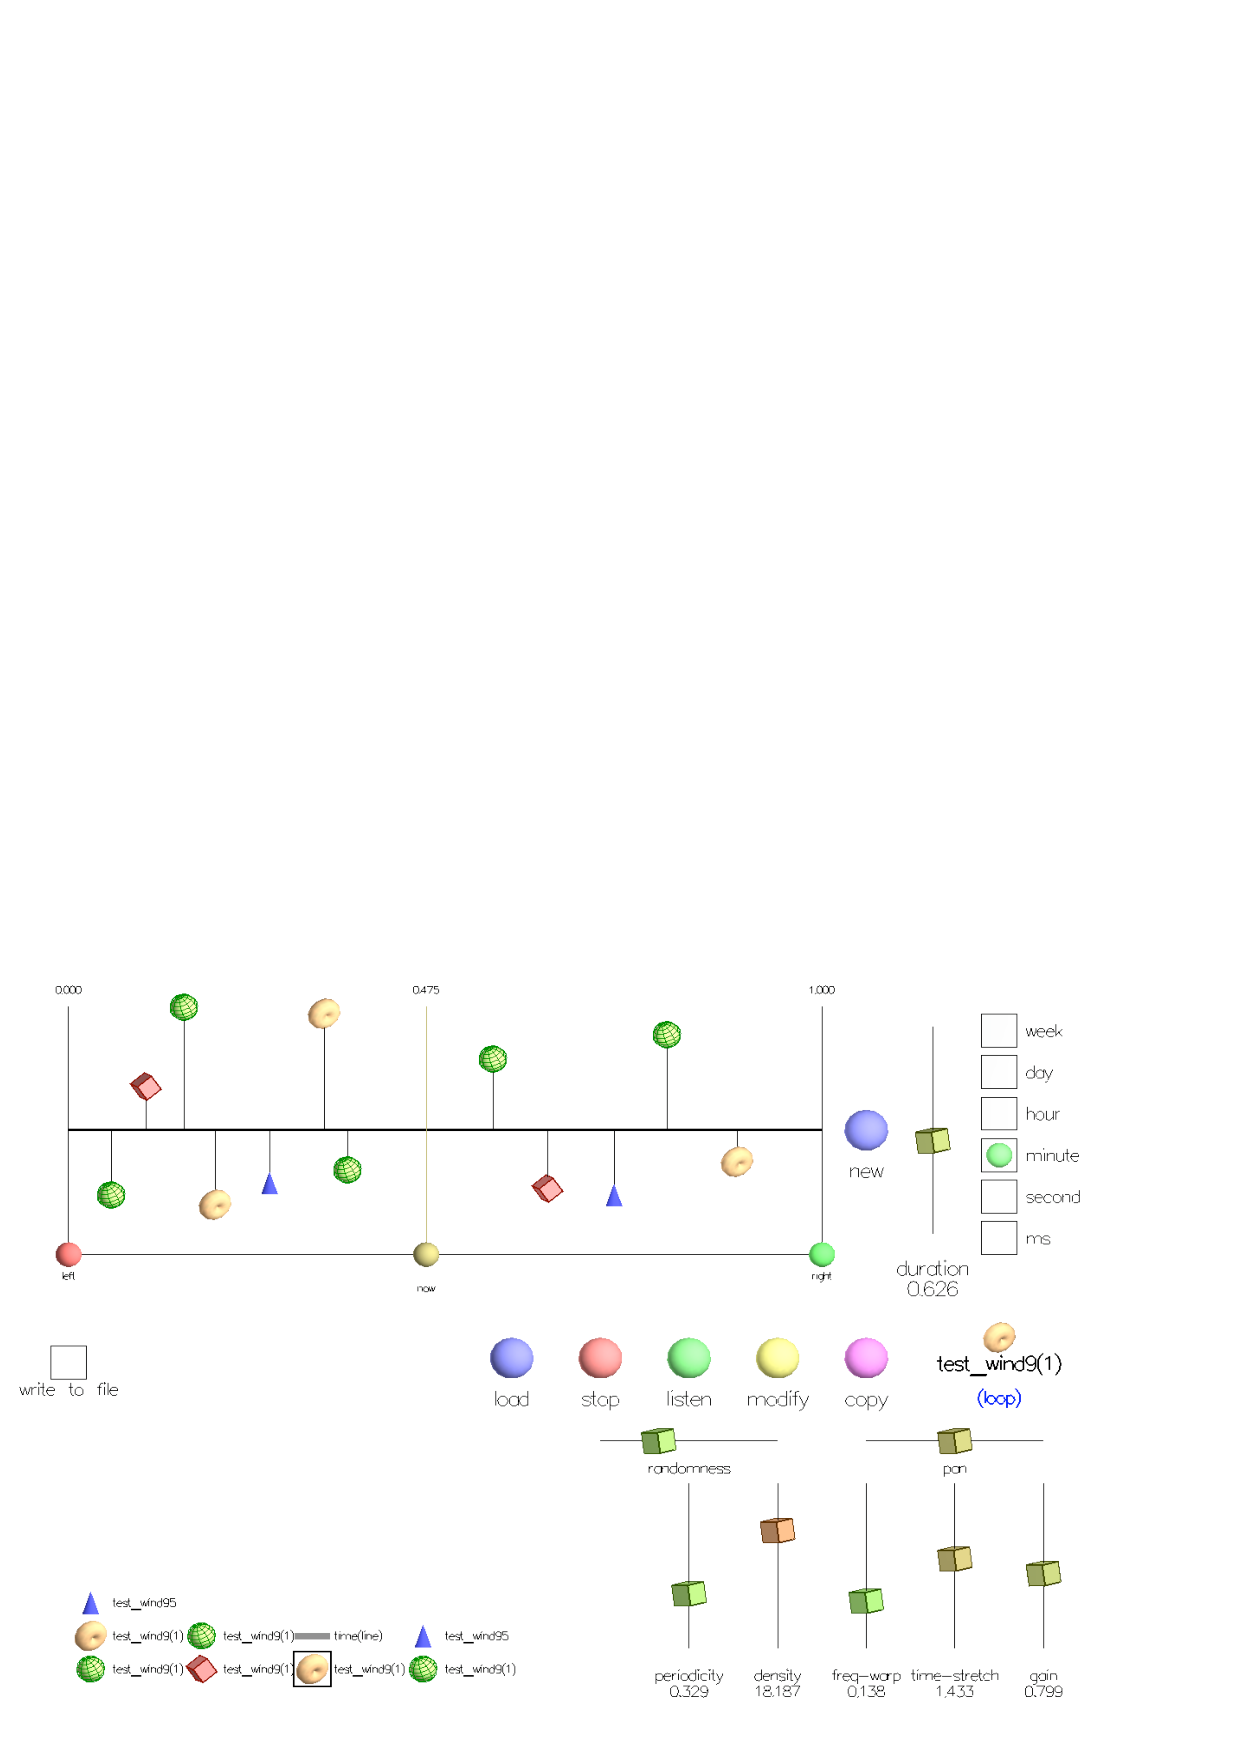
\includegraphics[width=1\columnwidth]{ui_synthesis.pdf}
    \caption{Screenshot of transformation + synthesis interface.}  
%    Templates from the library
 %   (lower left) can be controlled in real-time (lower-right) and be placed on timelines (above).} 
    \label{fig:ui_synthesis}
  \end{center}
\end{figure}

\subsection{Deterministic Events} 

Deterministic events are synthesized from their tracks via sinusoidal
re-synthesis. Frequency and magnitude between consecutive frames in a
track are linearly interpolated, and time-domain samples are computed
from this information. 

The track representation allows considerable flexibility in applying
frequency and time transformations on a deterministic event. The event's
frequency can be linearly scaled before computing
the time-domain samples, by multiplying the frequency at each point on
its tracks by a specified factor. Similarly, the event can be stretched
or shrunk in time by scaling the time values in the time-to-frequency
trajectories of its tracks. This works for almost any
frequency or time scaling factor without producing artifacts. Frequency
and time transformations can take place in real-time in TAPESTREA, 
allowing an event to be greatly stretched, shrunk or pitch shifted even
as it is being synthesized.

\begin{figure}[h]
  \begin{center}
%    \framebox[7cm]{\rule[-5mm]{0cm}{5cm} }
    \includegraphics[width=1\columnwidth]{ui_library.pdf}
    \caption{Library of saved templates.} 
    \label{fig:ui_library}
  \end{center}
\end{figure}

\subsection{Transient Events} 

Since transient events are brief by definition, TAPESTREA stores them
directly as time-domain audio frames. Synthesizing a transient event
without any transformations, therefore, involves playing back the
samples in the audio frame. 

In addition, TAPESTREA allows time-stretching and pitch-shifting in
transient events as well. This is implemented using a phase
vocoder~\cite{Dolson86}, which limits the scaling factors to a range smaller
and perhaps more reasonable than what is available for deterministic events,
yet large enough to create noticeable effects.

Transient events by nature can also act as ``grains'' for traditional
granular synthesis~\cite{Truax90,Roads02}. The
transformation tools for transients, along with the
additional synthesis templates described in Sections 4.4 to 4.6, can
thus provide an interactive ``granular synthesis'' interface.

\subsection{Stochastic Background}

The internal representation of a \textit{stochastic background} template
begins with a link to a sound file containing the related background
component extracted in the analysis phase. However, merely looping
through this sound file or randomly mixing segments of it does not
produce a satisfactory background sound. Instead, our goal here is to
generate ongoing background that sounds controllably similar to the
original extracted stochastic background. 

Therefore, the stochastic background is synthesized from the saved sound
file using an extension of the wavelet tree learning
algorithm~\shortcite{Dubnov02}. In the original algorithm, the saved
background is decomposed into a wavelet tree where each node
represents a coefficient, with depth corresponding to resolution.
The wavelet coefficients are computed using the Daubechies wavelet with 5
vanishing moments. A new wavelet tree is then constructed, with each node selected
based on the similarity of its ancestors and first \textit{k} predecessors to
corresponding sequences of nodes in the original tree. The learning
algorithm also takes into account the amount of randomness desired. Finally,
the new wavelet tree undergoes an inverse wavelet transform to provide the
synthesized time-domain samples. This learning technique works best with
the separated stochastic background as input, where the sinusoidal events it
would otherwise chop up have been removed.

TAPESTREA uses a modified and optimized version of the algorithm, which
follows the same basic steps but varies in details. For instance,
the modified algorithm includes the option of incorporating randomness
into the first level of learning, and also considers \textit{k} as
dependent on node depth rather than being constant.  More
importantly, it optionally avoids learning the coefficients at the
highest resolutions. These resolutions roughly correspond to high
frequencies, and randomness at these levels does not significantly alter
the results, while the learning involved 
takes the most time. Optionally stopping the learning at a lower level
thus optimizes the algorithm and allows it to run in real-time. 

Further, TAPESTREA offers interactive control over the learning
parameters in the form of ``randomness'' and ``similarity'' parameters. The
size of a sound segment to be analyzed as one unit can also be
controlled, and results in a ``smooth'' synthesized background for larger
sizes versus a more ``chunky'' background for smaller sizes. Creatively
manipulating these parameters can, in fact, yield interesting musical compositions generated through ``stochastic background''
alone.

\subsection{Event Loops}

Event loops (Figure \ref{fig:ui_loop_params}) are synthesis templates
designed to facilitate the parametric repetition of a single event. Any
deterministic or transient event template can be formed into a loop.
When the loop is played, instances of the associated event are
synthesized at the specified density and periodicity, and within a
specified range of random transformations. These parameters can be
modified while the loop is playing, to let the synthesized sound change
gradually. 

\begin{figure}[h]
  \begin{center}
%    \framebox[7cm]{\rule[-5mm]{0cm}{5cm} }
    \includegraphics[width=1\columnwidth]{ui_params.pdf}
    \caption{Sliders for controlling an event loop.} 
    \label{fig:ui_loop_params}
  \end{center}
\end{figure}

The density refers to how many times the event is repeated per second,
and could be on the order of 0.001 to 1000. At the higher densities, and
especially for transient events, the synthesized sound is often
perceived as continuous, thus resembling granular synthesis. 

The periodicity, ranging from 0 to 1, denotes how periodic the
repetition is, with a periodicity of 1 meaning that the event is
repeated at fixed time intervals. The interval between consecutive
occurrences of an event is generally determined by feeding the desired
periodicity and density into a Gaussian random number generator. It is
straightforward to replace this generator with one that follows a
Poisson or other user-specified probability distribution. 

In addition to the parameters for specifying the temporal placement of
events, TAPESTREA allows each instance of the recurring event to be
randomly transformed within a range. The range is determined by selected
average frequency- and time-scale factors, and a randomness factor that
dictates how far an individual transformation may vary from the average.
Individual transformation parameters are uniformly selected from within
this range. Apart from frequency and time scaling, the gain and pan of
event instances can also randomly vary in the same way.

\subsection{Timelines}

While a loop parametrically controls the repetition of a single event,
with some amount of randomization, a timeline allows a template to be
explicitly placed in time, in relation to other templates. Any number of
existing templates can be added to a timeline, as well as deleted from
it or re-positioned within it once they have been added. 

A template's location on the timeline indicates its onset time with
respect to when the timeline starts playing. When a timeline is played,
each template on it is synthesized at the appropriate onset time, and is
played for its duration or till the end of the timeline is reached. The
duration of the entire timeline can be on the order of milliseconds to
weeks, and may be modified after the timeline's creation. 

TAPESTREA also allows the placement of timelines within timelines (or
even within themselves). This allows for template placement to be
controlled at multiple time-scales or levels, making for a
``multiresolution synthesis.''

\subsection{Mixed Bags}

Another template for synthesis purposes is the mixed bag (Figure
\ref{fig:ui_mixedbag_params}), which is designed to control the relative
densities of multiple, possibly repeating, templates. Like a timeline, a
mixed bag can contain any number of templates, but these are randomly
placed in time and transformed, as in loops. The goal is to facilitate
the synthesis of a composition with many repeating components, without
specifying precisely when each event occurs. The real-time parameters
for controlling this also enable the tone of a piece to change over time
while using the same set of components, simply by synthesizing these
components differently. 

\begin{figure}[h]
  \begin{center}
%    \framebox[7cm]{\rule[-5mm]{0cm}{5cm} }
    \includegraphics[width=1\columnwidth]{ui_mixedbag.pdf}
    \caption{Sliders for controlling items in a mixed bag.} 
    \label{fig:ui_mixedbag_params}
  \end{center}
\end{figure}

When a template is added to a mixed bag, it can be set to play either
once or repeatedly. It also has a ``likelihood'' parameter, which
determines the probability of that template's being played in preference
over any of the other templates in the bag. Finally, it has a
``randomness'' parameter, which controls the range for random
transformations on that template, analogous to the randomness control in
event loops.

Beyond these individual template parameters, each mixed bag has overall
periodicity and density settings, which control the temporal
distribution of repeating templates in the same way that an event loop
does. However, while an event loop plays instances of a single event, a
mixed bag randomly selects a repeating template from its list whenever
it is time to synthesize a new instance. Templates with higher
likelihood settings are more likely to be selected for synthesis. 

%One way to think of a mixed bag is as a physical bag of marbles. The
%overall periodicity and density parameters determine how often someone
%dips his hand in the bag and pulls out a marble, or a template to be
%synthesized. The likelihood setting of a template or marble controls how
%likely it is for the hand to pull out that particular marble. A
%repeating marble is tossed back into the bag as soon as it has been
%drawn and observed (played). [THIS PARA COULD BE CUT OUT?]

\subsection{Pitch and Time Quantizations}

While sliders control the synthesis parameters in a continuous way, more
customized musical control can be exerted by quantizing pitches and
times to user-specified values. Pitch and time tables can be loaded
on-the-fly for each template. 

The frequency scaling factor of a template is quantized to the the
nearest entry in its pitch table, if it has one. 
%This directly
%influences the frequency at which a deterministic or transient event is
%synthesized. 
For event loops and mixed bags, this controls the possible
frequency scaling during random transformations on the underlying
events. The frequencies of individual templates on a timeline are
scaled, in the order in which they are played, by successive entries on
the timeline's pitch table. This allows a user-defined musical scale to
be applied to most templates. 

Rhythm can be similarly specified by quantizing time to the nearest
entry in a time table. In event loops and mixed bags, this quantizes the
event density parameter as well as the intervals between consecutive
events. On timelines, templates are positioned only at time points
corresponding to table entries, if a table exists. Thus, templates can
can start synthesizing at particular beats. 

\subsection{Score Language}

The manipulations described so far can be controlled via a
visual interface. Even finer control over the synthesis can be obtained
through the use of a score language. The audio programming language
ChucK~\cite{Wang03} is used here both for specifying precise
parameter values and for controlling exactly how these values change
over time.  Since ChucK allows the user to specify events and actions
precisely and concurrently \textit{in time}, it is straightforward to write
scores to dynamically evolve a sound tapestry.

A ChucK virtual machine is attached to TAPESTREA, which registers a
set of API bindings with which ChucK programs can access and control
sound templates and automate tasks.  Each script
(called a \textit{shred}) can be loaded as a sound template and be played
or put on timelines.  
%, like any other
Scripts can run in parallel, synchronized
to each other while controlling different parts of the synthesis.  Also, scripting
is an easy way to add ``traditional'' sound synthesis algorithms and real-time
control via MIDI and Open Sound Control.

\subsection{Other Controls}

TAPESTREA also offers some generic synthesis and playback controls. The gain and stereo panning of templates can be controlled individually, or randomly set by event loops and mixed bags. A reverb effect adapted from STK~\cite{Cook99} can also be added to the final synthesized sound.

The synthesis interface provides several ways to instantiate
new templates. Any existing template can be copied, while deterministic
and transient event templates can also be saved as event loops. New
timelines and mixed bags can be freely created, and existing templates
can be dragged onto or off these as needed. Templates can also be
deleted from the library, provided they are not being used in a timeline
or a mixed bag. Finally, while sound is generally synthesized in
real-time, TAPESTREA offers the option of writing the synthesized sound
to file.

\section{Discussion}

TAPESTREA makes it possible to create a wide range of {\it musical
tapestries}.  We describe one example recomposition here.  The
spectrogram (Figure \ref{fig:piece}) represents a 5 minute improvised
piece called \textit{Etude pour un Enfant Seul} (Study for a Child
Alone).  The source sound templates include the following: baby's cry
(1.5 sec; sinusoidal: 5 tracks), a clock chime (7 sec, sinusoidal: 25
tracks), glass breaking (.5 sec, sinusoidal: 4 tracks), car horn (.5
sec: sinusoidal: 10 tracks), bird chirp (.5 sec, sinusoidal: 4 tracks),
firework pop (.2 sec, transient), boom (.4 sec, transient), bang (.3
sec, transient).  These were extracted from BBC sound recordings. 
(Additional templates, including an ocean background with bird chirps
removed, were extracted but not used here.)

\begin{figure}[t]
  \begin{center}
%    \framebox[7cm]{\rule[-5mm]{0cm}{5cm} }
    \includegraphics[width=1\columnwidth]{piece.pdf}
    \caption{Example of a soundscape recomposition.  Diamonds represent areas of significant
     shift in the piece.} 
    \label{fig:piece}
  \end{center}
\end{figure}

We highlight some areas of interest in the recomposition (denoted by
numbered diamonds in Figure \ref{fig:piece}).  In area (1) are
time/frequency-warped instances of the baby (7x time-stretch, 0.5x
frequency-scaled), car horns (6x time, 0.2x and 0.28x freq), and glass
(4x time, 0.5x freq).  The percussion involving the pop/boom/bang
templates begins around (2) and is dynamically coordinated by scripts.
In (3), the percussion develops, punctuated by a solitary glass breaking
sound. At (4), greatly modified bird chirps (.15x time; 0.4x freq) fade
in as part of a periodic loop, which is so dense that chirps are
triggered at audio rates, forming a rich tone.  As time-stretch,
frequency-scale, and density are modified, the tone gradually morphs
into a flock of birds and back.  Combined with further modifications to
periodicity and randomness, the flock reaches its peak at (5), modeling
the sound of more than 30 birds spread out in time, frequency, volume,
and pan--all from a single bird chirp template.  The flock is then
manipulated to sparser texture, and the child returns at (6) with three
longer cries (baby cry; 9x time, 0.4x freq).

While this example makes good use of TAPESTREA, it is equally possible
to create completely differently styled compositions using the same tool
and even the same initial sounds.

\section{Conclusion} 

TAPESTREA is a technique and system for ``re-composing'' recorded sounds
by separating them into unique components and weaving these components
into \textit{musical tapestries}. The technique is applicable to musique
concr\`ete, soundscape composition and beyond, while the system combines
algorithms and interfaces for implementing the concepts. Key
contributions include: (1) an approach for recomposing natural sounds,
defining semantically clear {\it sound template} types linked to
specific processing techniques, (2) a system for extracting selected
sound components intro reusable templates, and for transforming and
synthesizing these, (3) a class of user interfaces aimed to facilitate
the process. 

Creating \textit{musical tapestries} with TAPESTREA is truly a
multidimensional process. The interface simultaneously provides visual
and audio information, while the system provides the means to
interactively extract sound components, transform them radically while
maintaining salient features, model them individually or in groups, and
synthesize the final multi-level ``recomposition'' in any number of
ways, ranging from a pre-set score to dynamically in real-time. Even
with a modest set of original sounds, there is no end to the variety of
{\it musical} tapestries one might weave. 

\center{
\texttt{http://taps.cs.princeton.edu/}
}

%\subsection{A Subsection}

%The Latex source, \textsf{icmc2006template.tex}, contains comments
%explaining how you should use Latex so as to conform to the paper
%format guidelines.

% \paragraph conforms to the guidelines; \subsubheading doesn't.
% I'll grant you that \paragraph is logically wrong, but it's easy.
%\paragraph{Third-order heading.}
%If you wish to use third-order headings, format them like this.  They
%start an unindented paragraph.

%Additional paragraphs are indented as usual.

%\subsection{References}

% We use chicago.(bst|sty), which supports (Author, year) cites and
% can be made to look _almost_ the way we wanted.  See chicago.sty
% for a list of all the flavors of citation you can do.
% \cite            (Laurel and Hardy 1932)
% \shortcite       (Laurel et al. 1932)
% \citeN           Laurel and Hardy (1932)
% \shortciteN      Laurel et al. (1932)

%Bibliographical references appear in parentheses; there is an example
%at the end of this sentence~\cite{canon}.  References with up to
%three authors include all the authors \cite{fugue}, but references
%with more than three authors use ``et al.''
% that is, you use \shortcite
%\shortcite{ircam-mw}.\footnote{Here is a footnote I hope you enjoy it.}
% (My naive attempt at hacking chicago.bst to do it had the side effect
% of leaving no space between the author and the "et".  We decided the
% italics were less than utterly indispensable.  If you know how to
% get them, though, drop me a note at eli@cs.cmu.edu.)

%A reference is not a subject or object. When you want to use the
%referenced work as part of a sentence, use the author or authors and
%use the year only for the reference, as in the following sentence:
% \citeN is "cite as noun"
%\citeN{mathews} includes a manual for Music V\@.  
% or if you want to, you can say
% Mathews~\citeyear{mathews} includes a manual for Music V\@.  

%Just for variety, this is a reference to an ICMC
%paper~\cite{superscalar}.

%\subsection{Figures and Captions}

%Place all figures in-line with the text.  Please include an
%explanatory caption for each.

%\begin{figure}[htbp]
%  \begin{center}

%    \framebox[7cm]{\rule[-5mm]{0cm}{5cm} }

%    \caption{This figure intentionally left blank.} 
%    \label{fig:emptybox}
%  \end{center}
%\end{figure}

%\section{Copyright Notices}

%You may wish to add a copyright notice to the bottom of the first
%column of your paper.  All copyrights remain with the authors.
%Authors will be asked to sign a form that gives ICMA, ICMC, and IEEE
%rights to sell the ICMC proceedings.  Typically, ICMC papers carry no
%explicit copyright notice.

% para from intro
%1. Existing composition techniques based on recordings of natural sounds
%are often time-domain-centric. Even with more spectrally oriented tools
%such as the phase vocoder, the source is a segment cut ``out of time''
%and can only be moderately transformed.  TAPESTREA allows the sound
%sculptor to select a region in both time and frequency, essentially
%specifying: ``Give me \textit{this} part of \textit{that} sound,'' to
%extract a reusable \textit{sound template}.  Furthermore, the system
%leverages the power of sinusoidal modeling to enable high-quality,
%potentially extreme transformation in time and frequency.

%TAPESTREA is a technique and system for re-composing natural
%(or any recorded) sounds into \textit{musical tapestries}.  It mediates
%and extends the ideas of musique concr\'ete and soundscapes with sound
%modeling techniques such as sinusoidal modeling and wavelet-tree texture
%synthesis.  The contributions are: (1) an approach for recomposing
%natural sounds, defining three types of \textit{sound templates}, each
%paired with the technique to which it's well-suited, (2) a
%system for selectively extracting sounds into reusable
%templates, and for flexibly transforming and synthesizing them, (3) a
%class of user interfaces aimed to facilitate the process.

%Creating \textit{musical tapestries} with TAPESTREA is truly a
%multidimensional process, providing the means to start with an existing
%sound, take it apart in meaningful ways, transform the subcomponents
%radically while maintaining their salient characteristics, model them
%individually and in groups, combine them with components from other
%sounds, score and synthesize the final "recomposition" or create an
%dynamic continuum of sound in real-time for installation or for
%performance.  There is no end to the variety of \textit{musical
%tapestries} one might weave, even with a very modest set of original
%sounds.

\bibliographystyle{chicago}
\small{
\bibliography{taps_icmc2006}
}

\end{document}
